\documentclass[xcolor=pdftex,dvipsnames,table]{beamer}
\usetheme[]{jku}
\usepackage{xcolor}
\usepackage{hyperref}
\usepackage{amsmath}
\usepackage{multirow} 
\usepackage{amsfonts}
\usepackage{amssymb}

\hypersetup{%
    colorlinks=false, linktocpage=false, pdfborder={0 0 0}, pdfstartpage=1, pdfstartview=FitV,%
    breaklinks=true, pdfpagemode=UseNone, pageanchor=true, pdfpagemode=UseOutlines,%
    plainpages=false, bookmarksnumbered, bookmarksopen=true, bookmarksopenlevel=1,%
    hypertexnames=true, pdfhighlight=/O,%hyperfootnotes=true,%nesting=true,%frenchlinks,%
    %for online viewing
    urlcolor=bioinfgreen, linkcolor=bioinfgreen, citecolor=bioinfgreen, %pagecolor=RoyalBlue,%
    % for printing
    %urlcolor=Black, linkcolor=Black, citecolor=Black, %pagecolor=Black,%
    pdftitle={Introduction},
    pdfauthor={\textcopyright\ Karin Schwarzbauer},
    pdfsubject={},
    pdfkeywords={},
    pdfcreator={pdfLaTeX},
}


\newcommand{\rcmd}[1]{{\tt{#1}}}
\newcommand{\rout}[1]{{\tt{#1}}}


\title{MACHINE LEARNING: THEORETICAL CONCEPTS UE}
\subtitle{Assignment 1: Maximum likelihood, Generalization Error}
\institute{Institute for Machine Learning}
\date{}
\partnerlogo{Logo_ML_modified_English}




\begin{document}

{ 
\setbeamertemplate{footline}{}
\begin{frame}
  \maketitle
\end{frame}
}


\begin{frame}{Contact}
\textbf{LVA Head: Johannes Brandstetter, Johannes Kofler }\\
\textbf{Staff:} M. Holzleitner, J. Arjona-Medina, A. Mayr, T. Adler, \\ H. Ramsauer \\ 
------------\\
Institute for Machine Learning\\
Johannes Kepler University\\
Altenberger Str.~69\\
A-4040 Linz\\
------------\\
E-Mail: \href{mailto:theoretical@ml.jku.at}{\tt theoretical@ml.jku.at}\\
\textbf{Only mails to this list are answered!} \\
\href{https://www.jku.at/en/institute-for-machine-learning/}{Institute Homepage}

\end{frame}


\begin{frame}{Generalization Error}
	\par
	\scriptsize
	\textcolor{NavyBlue}{Supervised learning:\\} 
	\begin{itemize}
		\item some real world process produces data  $\mathbf{x} \in \mathbb{R}^d$
		\item to every data point we want to infer a $y \in \mathbb{R}$ that is either a category (classification) or a value (regression)
		\item for a set of data points $X = \{\mathbf{x}^1, \ldots, \mathbf{x}^l\}$ we know the associated $\{y^1, \ldots, y^l\}$
		\item we call $\{ \mathbf{z}^1, \ldots, \mathbf{z}^l\ \}$ the training data, where $\mathbf{z}^i = (\mathbf{x}^i, y^i)$
	\end{itemize}
	
	\textcolor{NavyBlue}{What does it mean to learn from data? \\} 
	\begin{itemize}
		\item learning is model selection
		\item supervised learning: select a model that minimizes the prediction error on future data
		\item i.e. we want our model to generalize from the training data to future data
	\end{itemize}
\end{frame}
%-------------------------------------------------------------------------------




\begin{frame}{Generalization Error}
	\par
	\scriptsize
	\textcolor{NavyBlue}{What does it mean to learn from data? More formal: \\}
	\begin{itemize}
		\item selecting a model, i.e. a function $g(\mathbf{x})$ that associates $y$ to input $\mathbf{x}$
		\item if the model is parametrized with an vector $\mathbf{w}$ we write $g(\mathbf{x}; \mathbf{w})$
		\item we want to select a "good" model (i.e. good parameters)% if it is a parameterized model)
		\item we measure the performance of our model with a loss function $L(y, g(\mathbf{x}; \mathbf{w}))$
	\end{itemize}
	\textcolor{NavyBlue}{Typical loss functions \\}
	\begin{itemize}
	 	\item zero-one-loss\\$L(y,g(\mathbf{x};\mathbf{\omega})) =  \begin{cases}0 & \text{for } y=g(\mathbf{x};\mathbf{\omega})\\1 & \text{for } y\ne g(\mathbf{x};\mathbf{\omega}) \end{cases}$
	 	\item quadratic loss \\ $L(y,g(\mathbf{x};\mathbf{\omega})) = (y-g(\mathbf{x};\mathbf{\omega}))^2$
	 \end{itemize}
\end{frame}
%-------------------------------------------------------------------------------


\begin{frame}{Generalization Error}
		\par
		\scriptsize
		\textcolor{NavyBlue}{What does it mean to generalize? \\}
		\begin{itemize}
			\item the \textbf{generalization error} which is the \textbf{expected loss on future data} should be as low as possible
			\item the generalization error, also called the risk $R$ is the functional:
		\end{itemize}
		
		\begin{equation*}
		R(g(.;\mathbf{w})) \ = \ E_{\mathbf{z}} \left(L(y,g(\mathbf{x};\mathbf{w})) \right) =  \int_Z L(y,g(\mathbf{x};\mathbf{w})) \ p(\mathbf{z}) \ d\mathbf{z}
		\end{equation*}
		where $p(\mathbf{z})$ denotes the probability of $\mathbf{z}$ and $Z$ is the set of all future $\mathbf{z}$.
		
		%Note: The risk for the quadratic loss might already be familiar to you. It is called the  "mean squared error".	
		
		\textcolor{NavyBlue}{Since we don't have all future data, we need to approximate the risk\\}
		\begin{itemize}
			\item we choose $m$ samples from $\{ \mathbf{z}^1, \ldots, \mathbf{z}^l\ \}$ 
			\item this is the so called "test set" $\{ \mathbf{z}^1, \ldots, \mathbf{z}^m\ \}$, $m < l$
			\item assuming the $\mathbf{z}$ are iid and $m$ is large enough we can approximate the risk 
		\end{itemize}		
		
		\begin{equation*}
				R(g(.;\mathbf{w})) \approx \frac{1}{m} \sum_{i=1}^{m}   \left(L(y^i,g(\mathbf{x}^i;\mathbf{w})) \right)
		\end{equation*}
			
\end{frame}
%-------------------------------------------------------------------------------


%\begin{frame}{Loss functions}
% \begin{itemize}
%  \item zero-one-loss\\$L(y,g(\mathbf{x};\mathbf{\omega})) =  \begin{cases}0 & \text{for } y=g(\mathbf{x};\mathbf{\omega})\\1 & \text{for } y\ne g(\mathbf{x};\mathbf{\omega}) \end{cases}$
%  \item quadratic loss \\ $L(y,g(\mathbf{x};\mathbf{\omega})) = (y-g(\mathbf{x};\mathbf{\omega}))^2$
%   \end{itemize}
%\end{frame}
%-------------------------------------------------------------------------------




\begin{frame}{Empirical Estimation of Risk}
  	\par
  	\scriptsize
  	\textcolor{NavyBlue}{If we don't have much data: \\}
  	\begin{itemize}
  		\item Cross Validation: using folds of the data
  	\end{itemize}
    \begin{figure}[ht!]
    	 \centering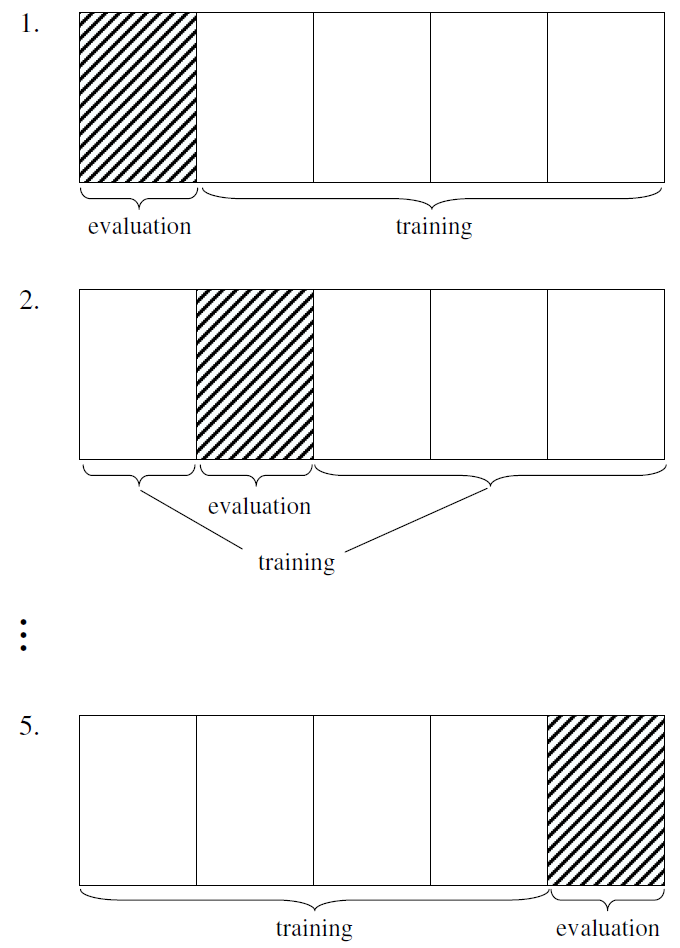
\includegraphics[width=0.3\textwidth]{figure2-2.png}
	\end{figure}
    CV risk is an almost unbiased estimator for the risk
\end{frame}
%-------------------------------------------------------------------------------

\begin{frame}{Minimal Risk for Gaussian Classification}
	\par
	\scriptsize
	\textcolor{NavyBlue}{Density function of multivariate Gaussian:}
	\begin{equation*}
		 \mathcal{N}(\mathbf{x}; \mathbf{\mu}, \mathbf{\Sigma}) = \ \frac{1}{\left( 2 \ \pi \right)^{d/2} \left| \mathbf{\Sigma} \right|^{1/2}} \ e^{ - \frac{1}{2} \ (\mathbf{x}-\mathbf{\mu})^T \ \mathbf{\Sigma}^{-1} (\mathbf{x}-\mathbf{\mu})}
	\end{equation*}
	\textcolor{NavyBlue}{Classification task where the data for each class is drawn from a Gaussian\\}
	 %\vspace{6pt}
	 \begin{itemize}
		\item $p(\mathbf{x} \vert y=1) \propto \mathcal{N} (\mathbf{\mu}_1 , \mathbf{\Sigma}_1 ) $
		%\vspace{6pt}
		\item $p(\mathbf{x} \vert y=-1) \propto \mathcal{N} (\mathbf{\mu}_{-1} , \mathbf{\Sigma}_{-1} ) $
		%\vspace{6pt}
	 \end{itemize}

	 \begin{minipage}{0.7\textwidth}
		 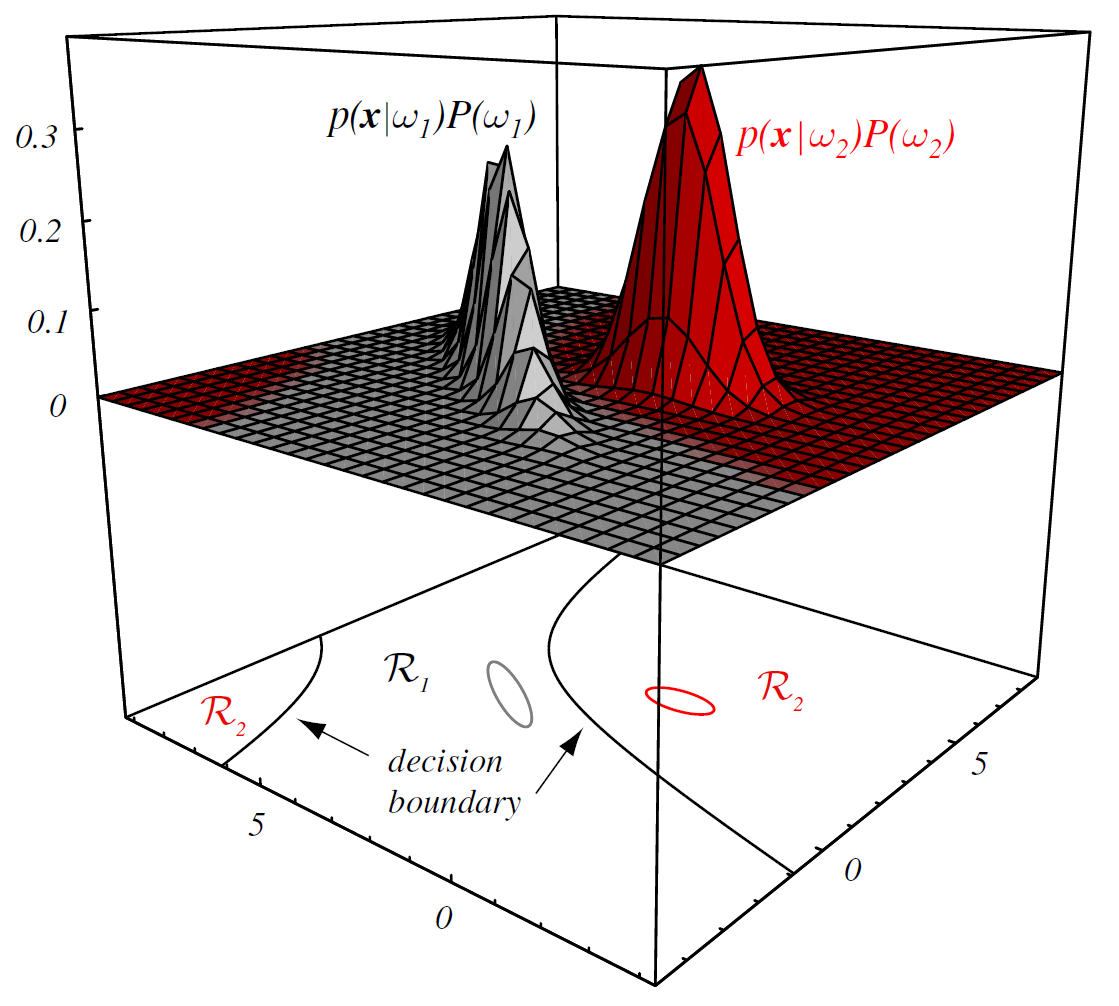
\includegraphics[angle=0,width=0.7\textwidth]{figure2-4.png}
	 \end{minipage}%
	 \begin{minipage}{0.3\textwidth} 
		 \tiny {A two-dimensional
		 classification task where the data for each class are drawn from a
		 Gaussian (black: class 1, red: class -1). The optimal decision
		 boundaries are two hyperbolas. Here $\omega_1 \ \equiv \ y = 1$ and
		 $\omega_2 \ \equiv \ y = -1$. In the gray regions $p(y=1 \mid \mathbf{x}) \
		 > \ p(y=-1 \mid \mathbf{x})$ holds and in the red regions the opposite
		 holds. Copyright \copyright\ 2001 John Wiley \& Sons, Inc.}
	 \end{minipage}
\end{frame}
%-------------------------------------------------------------------------------

%\begin{frame}{Minimal Risk for Gaussian Classification}
%\begin{figure}
%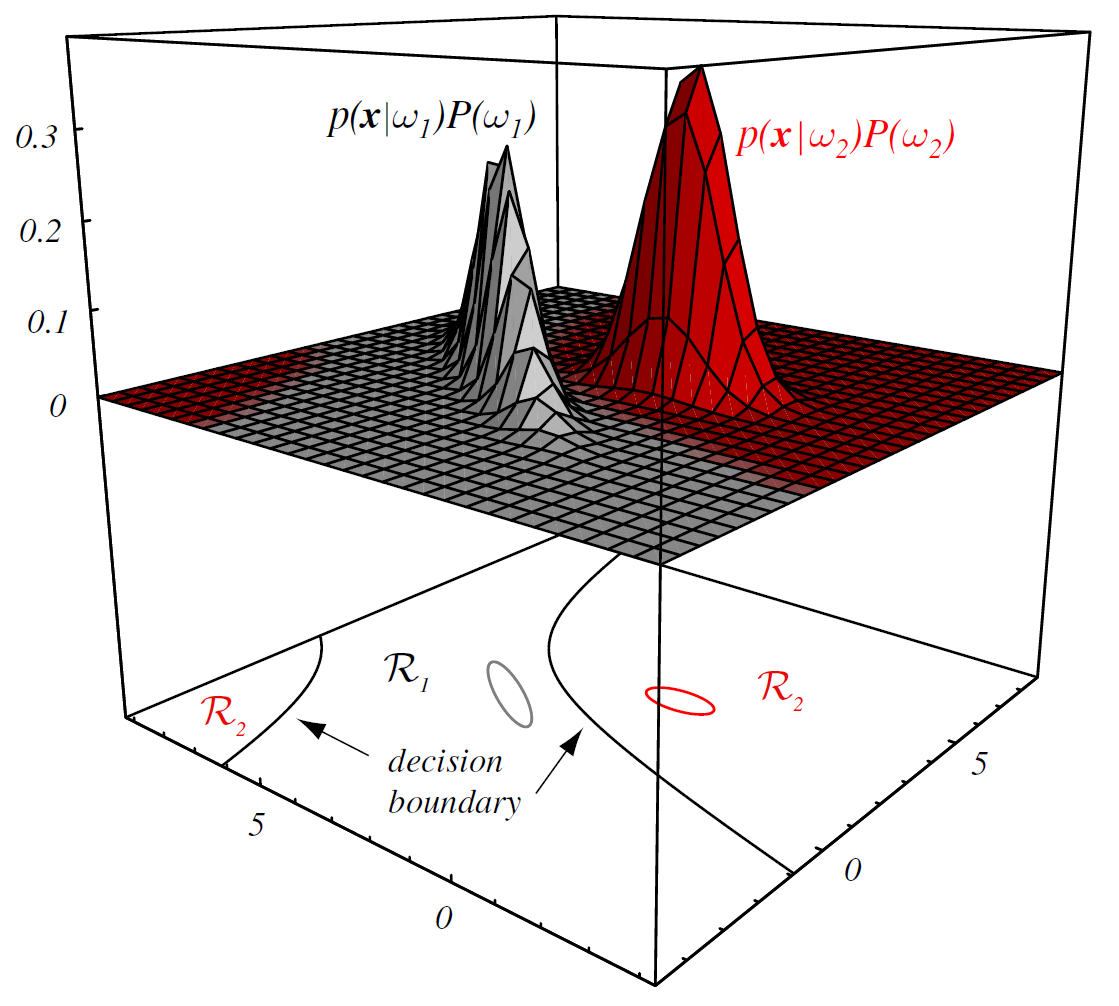
\includegraphics[angle=0,width=0.5\textwidth]{figure2-4.png}
%\caption{\tiny A two-dimensional
%classification task where the data for each class are drawn from a
%Gaussian (black: class 1, red: class -1). The optimal decision
%boundaries are two hyperbolas. Here $\omega_1 \ \equiv \ y = 1$ and
%$\omega_2 \ \equiv \ y = -1$. In the gray regions $p(y=1 \mid \mathbf{x}) \
%> \ p(y=-1 \mid \mathbf{x})$ holds and in the red regions the opposite
%holds. Copyright \copyright\ 2001 John Wiley \& Sons, Inc.}
%\end{figure}
%\end{frame}

\begin{frame}{Minimal Risk for Gaussian Classification}
	\par
	\scriptsize
	\textcolor{NavyBlue}{We define the regions}
	\begin{itemize}
		\item of class 1 as $X_1 \ = \ \{ \mathbf{x} \mid g(\mathbf{x}) > 0 \}$
		\item of class -1 as $X_{-1} \ = \ \{ \mathbf{x} \mid g(\mathbf{x}) < 0 \} $
	\end{itemize}
	\textcolor{NavyBlue}{and the loss function as}
	\begin{eqnarray*}
		L(y,g(\mathbf{x};\mathbf{\omega})) \ = \ \left\{
		\begin{array}{lll}
			0 & \mbox{for} & y \cdot g(\mathbf{x};\mathbf{\omega}) > 0 \\
			1 & \mbox{for} & y \cdot g(\mathbf{x};\mathbf{\omega}) < 0
		\end{array} \right.
	\end{eqnarray*}
	\textcolor{NavyBlue}{Using the zero-one-loss we obtain for the risk} 
	\begin{equation*}
		\begin{split}
			R(g(.;\mathbf{\omega})) %& = \int_{X_1} \
			%p\left(\mathbf{x},y=-1\right) \ d\mathbf{x} \ + \  \ \int_{X_{-1}} \
			%p\left(\mathbf{x},y=1\right) \ d\mathbf{x} 
			& =
			\int_{X_1} \
				p\left(y=-1 \mid \mathbf{x} \right) \ p(\mathbf{x}) \ d\mathbf{x} \ + \  \ \int_{X_{-1}} 
				\ p\left(y=1 \mid \mathbf{x} \right)  \ p(\mathbf{x}) \ d\mathbf{x} \\ & =
			\int_{X} \left\{ \begin{array}{lll}
					p\left(y=-1 \mid \mathbf{x} \right) & \mbox{for} & g(\mathbf{x}) > 0 \\
					p\left(y=1 \mid \mathbf{x} \right) & \mbox{for} & g(\mathbf{x}) < 0
				\end{array} \right\}
				\ p(\mathbf{x}) \ d\mathbf{x} \ .
		\end{split}
	\end{equation*}
\end{frame}
%-------------------------------------------------------------------------------

\begin{frame}{Minimal Risk for Gaussian Classification}
	\fontsize{8}{3.1}\selectfont
	\vspace{12pt}
	\textcolor{NavyBlue}{Risk can be minimized by}
	\begin{itemize}
		\item choosing the smaller value of $p\left(y=-1 \mid \mathbf{x} \right)$ and $p\left(y=1 \mid \mathbf{x} \right)$.
	\end{itemize}
	 \textcolor{NavyBlue}{Therefore, risk is minimal if}
	\begin{eqnarray*}
		\label{eq:minrisk} g(\mathbf{x};\mathbf{\omega}) \ \left\{
		\begin{array}{lll}
		> \ 0 & \mbox{for} &  p\left(y=1 \mid \mathbf{x} \right) \ > \
		p\left(y=-1 \mid \mathbf{x} \right)\\
		< \ 0 & \mbox{for} & p\left(y=-1 \mid \mathbf{x} \right) \ > \ p\left(y=1
		\mid \mathbf{x} \right)
		\end{array} \right. 
	\end{eqnarray*}
	
	\textcolor{NavyBlue}{The minimal risk is}
	\begin{equation*}
		 \begin{split}
			R_{\mathrm{min}} %& =  \int_{X}  \min\{ p\left(\mathbf{x},y=-1\right), p\left(\mathbf{x},y=1\right) \} \ d\mathbf{x} \\
			                 & =\int_{X}  \min\{ p\left(y=-1 \mid \mathbf{x} \right), p\left(y=1 \mid \mathbf{x}\right) \} \ p(\mathbf{x}) \ d\mathbf{x} 
		\end{split}
	\end{equation*}
\end{frame}
%-------------------------------------------------------------------------------

\begin{frame}{Discriminant Function}
	\par
	\scriptsize
	\textcolor{NavyBlue}{A discriminant function which minimizes the future risk is}
	\begin{equation*}
		\begin{split}
			g(\mathbf{x}) & = \ p(y=1 \mid \mathbf{x} ) \ - \  p(y=-1 \mid \mathbf{x} ) \\
			              & = \frac{1}{p(\mathbf{x})} \left( \ p(\mathbf{x} \mid y=1) \  p(y=1) \ - \ p(\mathbf{x} \mid y=-1) \  p(y=-1) \ \right) \ ,
		\end{split}
	\end{equation*}
	
	\begin{itemize}
		\item only the difference in the last brackets matters because $p(\mathbf{x}) >0$
		\item optimal discriminant function is not unique since difference of strict monotone mappings of $ p(y=1
		\mid \mathbf{x} )$ and $p(y=-1 \mid \mathbf{x} )$ keep the sign 
	\end{itemize}

	Take the logarithm $\rightarrow$ more convenient discriminant function which also
	minimizes the future risk:
	%\begin{eqnarray*}
	\begin{equation*}
		\begin{split}
			g(\mathbf{x}) & = \ln p(y=1 \mid \mathbf{x} ) \ - \  \ln p(y=-1 \mid \mathbf{x} ) \\
				          & = \ln \frac{ p(\mathbf{x} \mid y=1)}{p(\mathbf{x} \mid y=-1)} \ + \ \ln \frac{ p(y=1)}{ p(y=-1)} \ .
		\end{split}
	\end{equation*}
\end{frame}


\begin{frame}{Discriminant Function for Gaussian Classific.}
	\par
	\scriptsize
	\begin{equation*}
		\begin{split}
			g(\mathbf{x}) & =
			- \frac{1}{2} \ (\mathbf{x}-\mathbf{\mu}_1)^T \ \mathbf{\Sigma}_{1}^{-1} (\mathbf{x}-\mathbf{\mu}_1)
			\ - \ \frac{d}{2} \ln 2 \pi \ - \frac{1}{2} \ \ln
			\left| \mathbf{\Sigma}_1 \right| \ + \ln p(y=1) \\ 
			& \quad  + \frac{1}{2}
			\ (\mathbf{x}-\mathbf{\mu}_{-1})^T \ \mathbf{\Sigma}_{-1}^{-1} (\mathbf{x} -\mathbf{\mu}_{-1}) + \
			\frac{d}{2} \ln 2 \pi \ + \  \frac{1}{2} \ \ln \left| \mathbf{\Sigma}_{-1}
			\right| \ - \ \ln p(y=-1) \\ 
			& = - \frac{1}{2} \
			(\mathbf{x}-\mathbf{\mu}_1)^T \ \mathbf{\Sigma}_{1}^{-1} (\mathbf{x}-\mathbf{\mu}_1) \ - \  \frac{1}{2} \ \ln
			\left| \mathbf{\Sigma}_1 \right| \ + \ \ln p(y=1) \\ & 
			\quad + \frac{1}{2}
			\ (\mathbf{x}-\mathbf{\mu}_{-1})^T \ \mathbf{\Sigma}_{-1}^{-1} (\mathbf{x}-\mathbf{\mu}_{-1}) \ + \
			\frac{1}{2} \ \ln \left| \mathbf{\Sigma}_{-1} \right| \ - \ \ln p(y=-1) \\  
			& =  - \frac{1}{2} \mathbf{x}^T \left( \mathbf{\Sigma}_{1}^{-1} \ - \
			\mathbf{\Sigma}_{-1}^{-1} \right) \ \mathbf{x} \ + \  \mathbf{x}^T \left( \mathbf{\Sigma}_{1}^{-1}
			\mathbf{\mu}_1   \ - \ \mathbf{\Sigma}_{-1}^{-1} \mathbf{\mu}_{-1}\right) \ -
			\frac{1}{2} \ \mathbf{\mu}_1^T \mathbf{\Sigma}_{1}^{-1} \mathbf{\mu}_1 \\
			& \quad + \frac{1}{2} \ \mathbf{\mu}_{-1}^T  \mathbf{\Sigma}_{-1}^{-1} \mathbf{\mu}_{-1}
			\ - \  \frac{1}{2} \ \ln \left| \mathbf{\Sigma}_1 \right| \ + \  \frac{1}{2} \
			\ln \left| \mathbf{\Sigma}_{-1} \right| \ +\ln p(y=1) \  - \ \ln
			p(y=-1) \\
			& =  - \frac{1}{2} \mathbf{x}^T \mathbf{A} \mathbf{x} \ + \  \mathbf{w}^T
			\mathbf{x} \ + \ b \ .
		\end{split}
	\end{equation*}
\end{frame}


%\begin{frame}{Discriminant Function for Gaussian Classific.}
%\fontsize{8}{7.2}\selectfont
%\begin{eqnarray*}
%&&g(\mathbf{x}) \ = \
% - \frac{1}{2} \ (\mathbf{x}-\mathbf{\mu}_1)^T \ \mathbf{\Sigma}_{1}^{-1} (\mathbf{x}-\mathbf{\mu}_1)
%\ - \ \frac{d}{2} \ln 2 \pi \ - \\\nonumber &&\frac{1}{2} \ \ln
%\left| \mathbf{\Sigma}_1 \right| \ + \ \ln p(y=1) \ + \\\nonumber &&\frac{1}{2}
%\ (\mathbf{x}-\mathbf{\mu}_{-1})^T \ \mathbf{\Sigma}_{-1}^{-1} (\mathbf{x}-\mathbf{\mu}_{-1}) \ + \
%\frac{d}{2} \ln 2 \pi \ + \  \frac{1}{2} \ \ln \left| \mathbf{\Sigma}_{-1}
%\right| \ - \ \ln p(y=-1) \ = \\\nonumber && - \frac{1}{2} \
%(\mathbf{x}-\mathbf{\mu}_1)^T \ \mathbf{\Sigma}_{1}^{-1} (\mathbf{x}-\mathbf{\mu}_1) \ - \  \frac{1}{2} \ \ln
%\left| \mathbf{\Sigma}_1 \right| \ + \ \ln p(y=1) \ + \\\nonumber &&\frac{1}{2}
%\ (\mathbf{x}-\mathbf{\mu}_{-1})^T \ \mathbf{\Sigma}_{-1}^{-1} (\mathbf{x}-\mathbf{\mu}_{-1}) \ + \
%\frac{1}{2} \ \ln \left| \mathbf{\Sigma}_{-1} \right| \ - \ \ln p(y=-1) \  =
%\\\nonumber && - \frac{1}{2} \mathbf{x}^T \left( \mathbf{\Sigma}_{1}^{-1} \ - \
%\mathbf{\Sigma}_{-1}^{-1} \right) \ \mathbf{x} \ + \  \mathbf{x}^T \left( \mathbf{\Sigma}_{1}^{-1}
%\mathbf{\mu}_1   \ - \ \mathbf{\Sigma}_{-1}^{-1} \mathbf{\mu}_{-1}\right) \ -
%\\\nonumber &&\frac{1}{2} \ \mathbf{\mu}_1^T \mathbf{\Sigma}_{1}^{-1} \mathbf{\mu}_1
% + \frac{1}{2} \ \mathbf{\mu}_{-1}^T  \mathbf{\Sigma}_{-1}^{-1} \mathbf{\mu}_{-1}
%\ - \  \frac{1}{2} \ \ln \left| \mathbf{\Sigma}_1 \right| \ + \  \frac{1}{2} \
%\ln \left| \mathbf{\Sigma}_{-1} \right| \ + \\\nonumber &&\ln p(y=1) \  - \ \ln
%p(y=-1) \  = \\\nonumber && - \frac{1}{2} \mathbf{x}^T \mathbf{A} \mathbf{x} \ + \  \mathbf{w}^T
%\mathbf{x} \ + \ b \ .
%\end{eqnarray*}
%\end{frame}

\begin{frame}{Maximum Likelihood}
	\par
	\scriptsize
	\textcolor{NavyBlue}{Quality criterion for our model:}
	\begin{itemize}
		\item in case of supervised learning: generalization error
		\item in case of unsupervised learning: Maximum Likelihood
	\end{itemize}
	
	\textcolor{NavyBlue}{Unsupervised setting:}
	\begin{itemize}
		\item \textbf{Given:}
			\begin{itemize} \scriptsize
				\item data samples $\{\mathbf{x} \} = \{\mathbf{x}^1, \ldots, \mathbf{x}^l\}$   (note: here $\mathbf{z}^i =  \mathbf{x}^i$, i.e. no labels!)
				\item a parametrized model distribution $p(\mathbf{x} ; \hat{\mathbf{w}})$ where $\hat{\mathbf{w}}$ are the parameters
			\end{itemize}  
		\item \textbf{Task:} find the parameter $\mathbf{w}$ that was most likely to produce this data.
		\item \textbf{Idea:} How likely was a given $\hat{\mathbf{w}}$ to produce the dataset? Assuming that the $\mathbf{x}$ are iid.:
	\begin{align*}
		\mathcal{L}(\{\mathbf{x}\}; \hat{\mathbf{w}}) = p(\{\mathbf{x}\};\hat{\mathbf{w}}) =  \prod_{i=1}^n p(\mathbf{x}^i ; \hat{\mathbf{w}})
	\end{align*}
	\item \textbf{Solution:} Find the $\mathbf{w}^*$ that maximizes $\mathcal{L}(\{\mathbf{x}\}; \hat{\mathbf{w}})$ %\\(or $\log \mathcal{L}(y)$, which is equivalent)
	\end{itemize}
\end{frame}


\begin{frame}{Maximum Likelihood}
	\par
	\scriptsize
	\textcolor{NavyBlue}{Find the $\mathbf{w}^*$ that maximizes $\mathcal{L}(\{\mathbf{x}\}; \hat{\mathbf{w}})$:}
	\begin{equation*}
		\mathbf{w}^* = \underset{ \hat{\mathbf{w}}}{arg \ max} \ \mathcal{L}(\{\mathbf{x}\}; \hat{\mathbf{w}}) = \underset{\hat{\mathbf{w}}}{arg \ max}\prod_{i=1}^n p(\mathbf{x}^i ; \hat{\mathbf{w}})
	\end{equation*}
	
	\textcolor{NavyBlue}{It is better to optimize a sum instead of a product: use log!}
	\begin{equation*}
		\mathbf{w}^* = \underset{ \hat{\mathbf{w}}}{arg \ max} \ log \ \mathcal{L}(\{\mathbf{x}\}; \hat{\mathbf{w}}) = \underset{\hat{\mathbf{w}}}{arg \ max}\sum_{i=1}^n log \ p(\mathbf{x}^i ; \hat{\mathbf{w}})
	\end{equation*}
\end{frame}


%\begin{frame}{Note on Programming Languages}
%\begin{itemize}
%\item this class will not teach you how to program
%\item We will provide hints for R
%\item For Python, use \texttt{NumPy/SciPy} and \texttt{Scikit-Learn}
%\item Use moodle-forum for questions
%\end{itemize}
%\end{frame}





\end{document}

